
\chapter{Bi-helical order and demixing in hybrid chiral LCs}
\chaptermark{Hybrid LCs: correlation effects}
\label{hybridLC2}


\begin{abstract}

We extend Onsager's theory to the case of hybrid molecular liquid crystals (LC) composed of colloidal particles immersed in thermotropic host. This framework enables us to explore colloid concentrations that are no longer infinitely small. Correlations between the colloids cause additional entropic and elastic contributions that interfere with surface anchoring effects explored in the previous chapter.  We consider two distinct regimes, namely weak coupling where surface anchoring only marginally impacts the colloid orientations and strong coupling where the typical realignments energy strongly exceeds the thermal energy. We demonstrate at weak coupling that collective colloidal effects driven by steric colloid-colloid interaction may lead to liquid-liquid phase separation between two biaxial fluid phases. In the strong coupling regime, we argue that elastic force may facilitate the formation bi-helical states where the helical organization of the colloidal and molecular components is unequal in pitch and even in handedness. 

\end{abstract}



\section{Introduction}

In the previous chapter we have studied  ordering of colloidal particles in so-called hybrid chiral liquid crystals composed of colloidal particles immersed in a low-molecular-weight cholesteric LC. Inspired by experimental work of we restricted our attention to the regime of low colloidal content where the principal ordering effect stem from single colloid properties related to surface anchoring and elastic distortions formed around the colloid surface. In this regime,  the average interparticle distance remains sufficiently large to guarantee that direct interactions between colloids, mediated by steric collisions or guided by some interference of surface defects, is unimportant. Raising the concentrations of colloids, which has not  been pursued in experiment thus far, offers interesting perspectives to explore the interplay between surface anchoring and alignment driven by colloid-colloid interactions as well as the role of (twist) elastic forces imparted by steric correlations between the colloids. In this chapter we generalize Onsager's theory suitably adapted to treat spatially non-uniform director field such as in a cholesteric, to explore the ordering of colloids at large concentrations where entropic and elastic contributions imparted by the colloids play a role. In doing so we consider two extreme cases, namely weak coupling where colloid realignemt cause by surface anchoring forces is weak, and strong coupling where such realignment is strong compared to the typical thermal fluctuations the colloid experience.  We highlight two main effects (i) surface-anchoring-driven  phase separation between two orthorhombic liquids at weak surface anchoring coupling and (ii) the formation of bi-helical chiral hybrid liquid crystals at large coupling strength.  Since the latter case should occur for both rods and discs alike exploring mixed molecular-colloidal LCs with inherent chirality opens up ways to create chiral fluids composed of discotic mesogens \cite{bisoyi2010discotic,bushby2002discotic}.   



\section{Second-virial density functional }

 With the single-colloid properties fully specified in the previous chapter, we now proceed towards describing the many-particle system by invoking a simple Onsager-type density functional theory \cite{Onsager}. The grand potential $\Omega$ of an assembly of colloids in the presence of an external  potential  reads in general form \cite{allenevans}:
 \begin{align}
 &  \Omega[\rho ]  = \int d \bfr d \bhu  \rho(\bfr, \bhu) \left [k_{B}T \ln {\mathcal V}   \rho(\bfr, \bhu)  +   U_{\rm ext}(\bfr, \bhu) - \mu  \right ] \nonumber \\
 & -\frac{k_{B}T}{2} \int d \bfr d \bhu \int d \bfr^{\prime} d \bhu^{\prime}  \rho(\bfr, \bhu)  \rho(\bfr^{\prime}, \bhu^{\prime}) \Phi(|\bfr - \bfr^{\prime}|, \bhu, \bhu^{\prime} )
 \label{grandpot}
 \end{align}
 with ${\mathcal V}$ denoting an effective thermal volume comprising contributions from rotational momenta and $\mu$ a chemical potential that controls the overall colloid concentration.  The first contribution describes an ideal gas of  non-interacting colloids while the second accounts for colloid-colloid interaction on the second-virial level. Here, the key input is the Mayer function $\Phi$  that, assuming the colloid interactions to be purely hard, renders minus unity if the cores of two colloids overlap and zero if they do not.

 We assume that the colloid positions remain randomly distributed. The orientational probability, however, will be affected by a helical rotation of  the  colloidal director field $\bn(z)$. Since the cholesteric pitch $\lambda \approx 30 \mu m$ is about an order of magnitude larger than the typical colloidal size (a few $\mu m$), the colloidal director is completely enslaved to the rotation of the local cholesteric director and adopts the same pitch length $\lambda$. A $\pi/2$ phase shift between the colloidal director $\bn(z)$ and the cholesteric one $\bn_{s}(z)$ may occur under certain anchoring conditions as we observe in Figs. 1 and 2.  This scenario may no longer hold at larger colloid concentrations and/or shorter cholesteric pitches where the twist elasticity of the colloids becomes considerable, as we will contemplate in a later section. Let us proceed by parameterizing the one-body density in terms of an overall density $\rho = N/V$ and an orientational probability that explicitly depends on the position $z$ along the helix:
 \beq
  \rho(\bfr, \bhu) = \rho f_{q}(\bhu \cdot \bn(z))
 \eeq
 In order to elaborate the grand potential we parameterize the system volume in cylindrical coordinates $d \bfr  = d \bfr_{\perp} dz$ with $0< |r_{\perp}| < \infty$ and $0< z < 2 \pi/q$. Given that the overall rod density is prescribed, the grand potential becomes a Helmholtz free energy $F$. The ideal (translation plus orientation) entropy  free energy per unit volume follow from:
  \begin{align}
 & \frac{ \beta F_{\rm id}}{ V} =  \int d \bhu \int_{0}^{2\pi}  \frac{d(qz)}{2 \pi} f_{q}( \bhu \cdot \bn(z))  \ln [{\mathcal V} \rho  f_{q}( \bhu \cdot \bn(z))]
 \end{align}
Since the orientational distribution does not change along the cholesteric director the ideal free energy density simplifies into the conventional form:
 \begin{align}
  \frac{ \beta F_{\rm id}}{ V} =  \rho \int d \bhu \ln [{\mathcal V} \rho  f_{q}( \bhu \cdot \bn)] f_{q}( \bhu \cdot \bn)
 \end{align}
 with $\bn$ denoting the local director along the helix. Similarly, the external potential in \eq{grandpot} is associated the surface anchoring free energy obtained from the Rapini-Papoular expression \eq{usurf}. It is  defined in the angular coordinates $\bhu(\theta, \delta)$ that co-rotate with the helical director so that:
\beq
\frac{F_{\rm s}}{V} = \rho \int d \bhu   f_{q}(\bhu \cdot \bn)  F_{s}(\bhu)
\eeq
Next, we introduce a linear coordinate transformation $z^{\prime} = z + \Delta z$ and write the excess free energy as follows:
  \begin{align}
  \frac{ \beta F_{\rm ex}}{ V}  = & \frac{\rho^{2}}{2} \int_{0}^{2 \pi}  \frac{d(qz)}{2 \pi}  \int d \bhu \int d \bhu^{\prime}  f_{q}( \bhu \cdot \bn(z)) \nonumber \\
  & \times \int_{-\lambda}^{\lambda} d \Delta z  {\mathcal A}(|\Delta z | , \bhu, \bhu^{\prime} ) f_{q}( \bhu^{\prime} \cdot \bn(z+\Delta z))
 \end{align}
 where  ${\mathcal A}$  is an orientation-dependent excluded {\em area} of rod or disc. The excess free energy is non-local since it depends on volume exclusion between a reference particle at $z$ and test particle  at $z+ \Delta z$ over which the local director will have rotated. It is therefore expedient to apply a transformation $\bhu^{\prime} \rightarrow \mathcal{R} (q\Delta z) \bhu^{\prime}$  which projects the orientation of the test colloid into the director frame of the reference one located at $z$ via the rotation matrix:
 \beq
 \mathcal{R} (q\Delta z)   =
  \begin{bmatrix}
     \cos(q\Delta z)  & \sin(q\Delta z) & 0   \\
   - \sin(q \Delta z) & \cos(q\Delta z) & 0  \\
   0 & 0 &  1  \\
      \end{bmatrix}  \nonumber
      \label{rota}
 \eeq
 The renders the excess free energy local so that it may be simplified into a compact form:
 \begin{align}
  \frac{ \beta F_{\rm ex}}{ V}  = & \frac{\rho^{2}}{2} \int d \bhu \int d \bhu^{\prime}  f_{q}( \bhu \cdot \bn) f_{q}( \bhu^{\prime} \cdot \bn) {\mathcal K}_{q}(\bhu, \bhu^{\prime})
 \end{align}
in terms of and excluded volume that takes into account the helical rotation of the director field:
\beq
 {\mathcal K}_{q}(\bhu, \bhu^{\prime}) =  \int_{-\lambda }^{\lambda} d \Delta z {\mathcal A}(|\Delta z | , \bhu, \mathcal{R}(q\Delta z)  \bhu^{\prime} )
\eeq
This clearly represents a highly convoluted object that we were only able to analyze analytically for thin hard rods, as discussed in the Appendix.
 As alluded to before, in the experimental situation the director twist is weak on the scale of the typical colloid size and it is justified to assume
\beq
 {\mathcal K}_{q}(\bhu, \bhu^{\prime}) \approx {\mathcal K}_{0}(\bhu, \bhu^{\prime}) =  v_{0}| \sin \gamma|
\eeq
which corresponds to the conventional excluded volume between two (infinitely) thin hard rods ($v_{0} = 2 L^{2}D$) or discs ($v_{0} = \tfrac{\pi}{2}D^{3}$), as per Onsager's original theory \cite{Onsager}. This approximation ignores any twist elastic resistance imparted by the colloids and should hold only for low to moderate colloid concentrations and weak director twist ($\lambda \gg L$ or $D$).  The effect of finite twist elasticity will be considered in an upcoming Section.


\begin{figure}
	\includegraphics[width = 0.8\columnwidth]{figures/chapter-4/fcorr3}
	\caption{ Unit-sphere projections of the local orientational probability of rods immersed in a low molecular-weight cholesteric phase at different surface anchoring strengths $\bar{W} = \beta W_{0}LD$, in the presence of a low-correlated colloidal liquid crystal composed by particles of the same kind.  The rod concentration represented here is  $c= \rho L^{2} D = 3$ which corresponds to an isotropic bulk system in the absence of surface anchoring. For all distributions, the rod-length-to-pitch is $qL=1$.}
	\label{fcorr3}
\end{figure}

   \begin{figure}
	\includegraphics[width = 0.8\columnwidth]{figures/chapter-4/fcorrd3}
	\caption{ Unit-sphere projections of the local orientational probability of discs immersed in a low molecular-weight cholesteric phase at different surface anchoring strengths $\bar{W} = \beta W_{0}D^2$, in the presence of a low-correlated colloidal liquid crystal composed by particles of the same kind.  The disc concentration represented here is  $c= \rho D^3 = 3$ which corresponds to an isotropic bulk system in the absence of surface anchoring. For all distributions, the disc-size-to-pitch is $qD=1$.}
	\label{fcorrd3}
\end{figure}
Combining all free energy contributions and formally minimizing the Helmholtz free energy with respect to $f_{q}$ yields a Boltzmann distribution similar to \eq{fsingle}:
   \beq
  f_{q}( \bhu ) = \mathcal{N} \exp \left (- \beta  F_{s} (\bhu) - \rho \int d \bhu^{\prime} f_{q}( \bhu^{\prime} ) {\mathcal K}_{0}(\bhu, \bhu^{\prime})  \right )
  \label{fcollec}
  \eeq
  which reduces to the ideal gas probability \eq{fsingle} for vanishing rod density $\rho = 0$ as it should. The above condition needs to be solved iteratively for a given combination of dimensionless parameters pertaining to the rods (discs), namely the  cholesteric pitch $qL$ ($qD$), surface anchoring strength $\beta W_{0}LD$ ($\beta W_{0}D^{2}$) and colloid concentration $c = \rho L^{2}D$ ($\rho D^{3}$). Possible phase transitions can be probed from the osmotic pressure $\Pi \equiv \partial F/\partial V|_{N,T}$ and chemical potential $\mu \equiv \partial F /\partial N|_{V,T}$ which read:
  \begin{align}
  \beta \Pi  &= \rho + \frac{\rho^{2}}{2} \langle \langle {\mathcal K}_{0}(\bhu, \bhu^{\prime}) \rangle \rangle _{f_{q}} \nonumber \\
  \beta \mu &= \ln [\rho v_{0}] + \langle \ln [f_{q} (\bhu)] + \beta F_{s}(\bhu)\rangle_{f_{q}} + \rho \langle \langle {\mathcal K}_{0}(\bhu, \bhu^{\prime}) \rangle \rangle_{f_{q}}
  \end{align}
  The  brackets are shorthand for an orientational average $ \langle  \cdot  \rangle_{f_{q}} = \int d \bhu   f_{q}(\bhu )(\cdot)$ measured with respect to the local director.


   \section{Orthorhombic liquid-liquid phase separation}

In the absence of surface anchoring realignment ($\bar{W} = 0$) the colloids undergo a conventional isotropic-uniaxial nematic transition. This is the classic Onsager scenario where an isotropic (I) phase  ($c_{I} = 4.19$, $S_{I} =0$) coexists with a (uniaxial) nematic phase  ($c_{N} = 5.34$, $S_{N} =0.792$). For $\bar{W} >0$ the $O(3)$ symmetry of the isotropic phase and the uniaxial $D_{\infty h}$ symmetry of the nematic will both be broken in favour of a biaxial, orthorhombic symmetry ($D_{2h}$), and a coexistence between two orthorhombic phases with different overall colloidal concentrations is expected. Resolving the coexistence conditions by imposing equality of chemical potential $\mu$ and pressure $\Pi$ in both phases we may explore phase diagrams in the surface anchoring amplitude - colloid concentration ($\bar{W} - c$) plane. The results are shown in \fig{phdiag} and demonstrate that a phase coexistence between two orthorhombic nematic phases is indeed possible in the weak coupling regime ($\bar{W} <1$). A critical point beyond which no phase transition is possible is located at a surface anchoring energy equivalent to a few times the thermal energy.

   \begin{figure}
	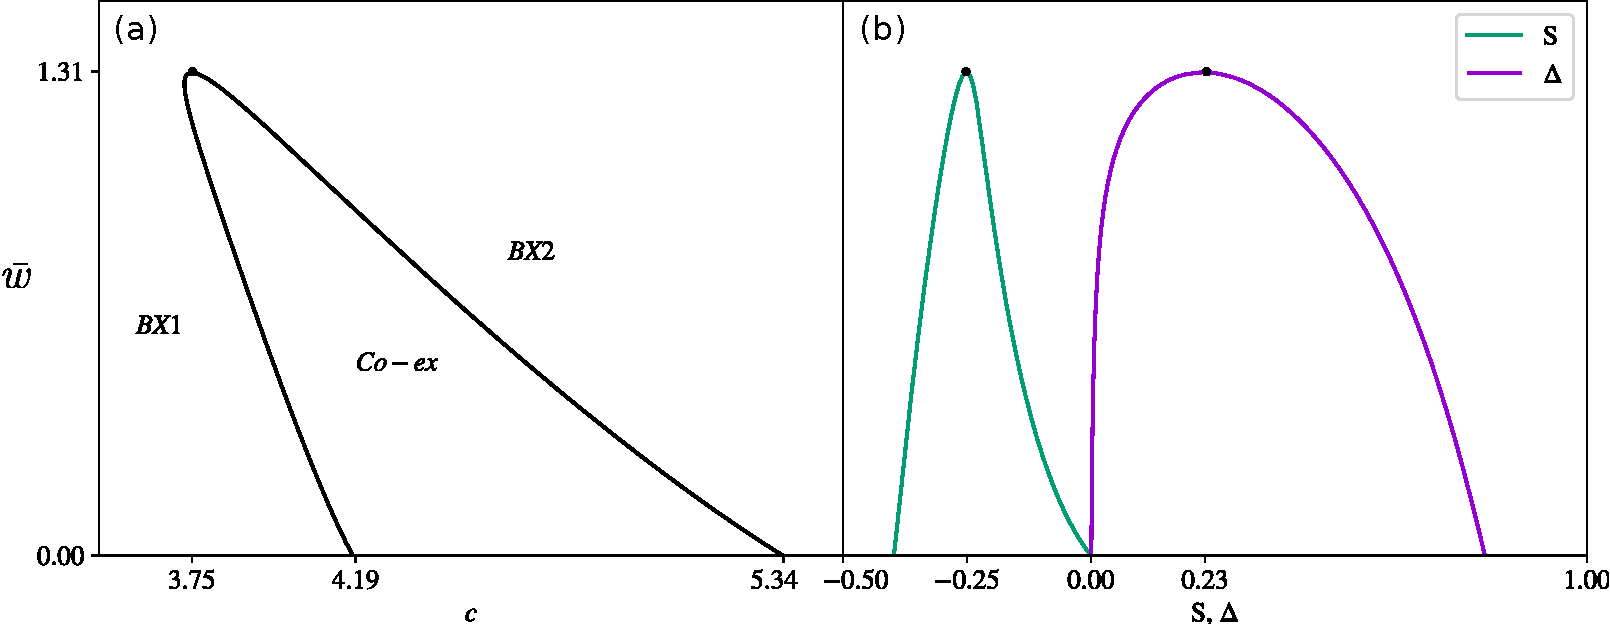
\includegraphics[width = \columnwidth]{figures/chapter-4/diagrams_q0.335_horizontal}
	\caption{(a) $\bar{W} - c $ phase diagram for rods with homeotropic or tangential surface anchoring, $qL = 0.335$. (b) Corresponding uniaxial (solid line) and biaxial (dashed line) nematic order. A qualitatively equivalent scenario can be found for discs with planar surface anchoring.}
	\label{phdiag}
\end{figure}


   \begin{figure}
	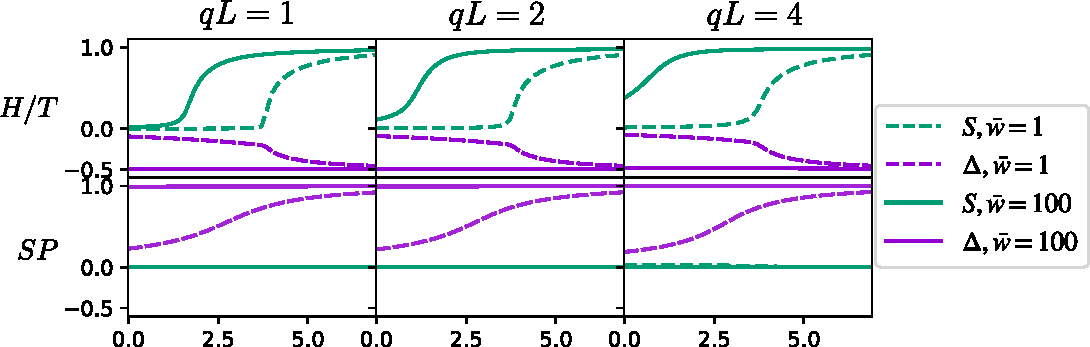
\includegraphics[width = \columnwidth]{figures/chapter-4/ordervsc_rods}
	\caption{ Uniaxial $S$ and biaxial $\Delta$ order parameters measured along the cholesteric nematic direction $\bn_{m}$ as a function of the concentration $c = \rho L^{2}D$ ($\rho D^{3}$) for rods at low (dashed lines) and high (solid lines) surface anchoring strength ($\bar{W} = \beta W_{0}LD = 1$ and $\bar{W} = \beta W_{0}LD = 100$ respectively) and three different values of $qL$.}
	\label{w1o}
\end{figure}

   \begin{figure}
	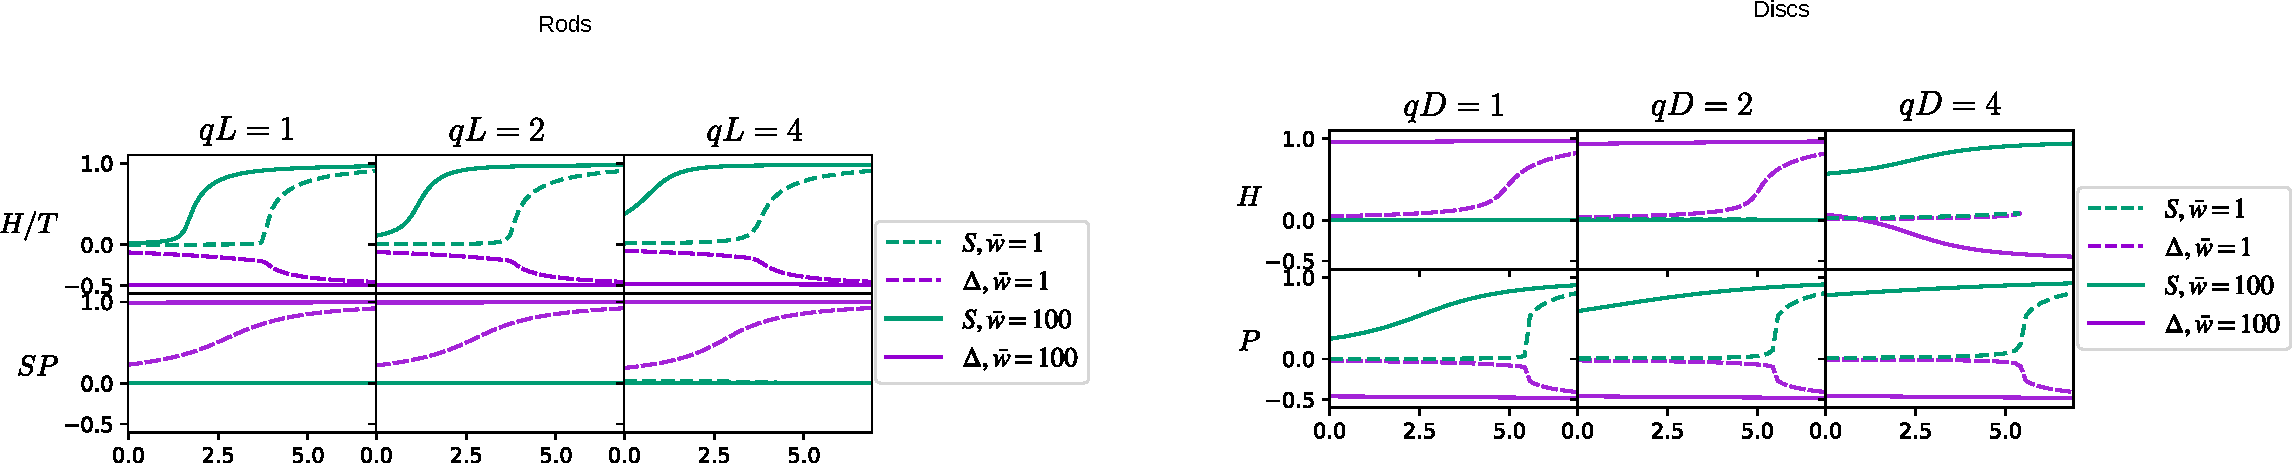
\includegraphics[width = \columnwidth]{figures/chapter-4/ordervsc_discs}
	\caption{ Uniaxial $S$ and biaxial $\Delta$ order parameters measured along the cholesteric nematic direction $\bn_{m}$ as a function of the concentration $c = \rho L^{2}D$ ($\rho D^{3}$) for discs at experimentally typical surface anchoring strength ($\bar{W} = \beta W_{0}D^2 = 1$ and $\bar{W} = \beta W_{0}D^2 = 100$ respectively) and three different values of $qL$.  The concentration range evaluated in the discotic homeotropic case for $\bar{W} = \beta W_{0}D^2 = 1$ is more restricted due to  numerical difficulties.}
	\label{w100o}
\end{figure}




\section{Effect of colloid-induced elasticity}

At certain conditions such as strong surface-anchoring coupling and large colloid concentration $\rho$ and short cholesteric pitches the twist elastic resistance generated by the anisotropic colloid-colloid repulsions will prevent the colloidal director from keeping pace with the rotation of the cholesteric director. This  may give rise to hybrid systems in which the colloidal director locally deviates from the the cholesteric helix. Let us attempt to explore this scenario in more detail starting from the cholesteric director field \eq{ns} that we keep fixed in the laboratory frame. In doing so, we rely on three further basic assumptions; (i) the colloids remain uniformly distributed throughout the system and do not affect the cholesteric helix whose  pitch $q$ remains unaffected, (ii)  the colloids are perfectly aligned and exhibit negligible thermal fluctuations around their main orientation, and (iii) the colloidal director remains perpendicular to the helical axis $\bz$ but we allow the degree of local twist to be non-uniform along the $z$-direction. We then parameterize the colloidal director as follows:
\beq
\bn(z) = \bx \cos \phi(z)   + \by \sin \phi(z)
\label{npara}
\eeq
 in terms of a local twist angle $\phi(z)$. Since the system is apolar, the director $\bn$ is equivalent to $-\bn$ so that $\phi(z)$ is equivalent to $\phi(z)  + \pi$.  For the cases discussed thus far, the colloidal director is simply co-helical with the cholesteric so that $\phi(z) =qz$ (mod $\pi )$.

 \subsection{Rods}

 Let us focus first on the case of rods. The fraction of rods aligned along the helical axis $\bz$ (as observed in \fig{fcorr3}) may be disregarded as they contribute very little to the twist elastic resistance imparted by the colloids. Since we assume that the rods are perfectly aligned along the above director we write the rod contour $\bfr_{{\mathcal S}}(t) = \bfr_{0} +  \frac{L}{2}t\bn(z)$ and applying this in the Rapini-Papoular expression \eq{usurf} along with the above parameterization we find:
\beq
F_{s}[\phi(z)]  = - \frac{1}{8} W_{0} LD \begin{cases}
       2 \pi \sin^{2}[\phi(z) -qz ] &  \textrm{H/T} \\
         4 \pi \cos^{2}[ \phi(z) - qz ]  &  \textrm{SP}
   \end{cases}
      \label{plahoms}
\eeq

In the absence of twist elastic effects the surface anchoring energy is indeed minimized along a uniform twist profile $\phi(z) = qz + \phi_{0} $ with phase shifts $\phi_{0} = \pi/2$ (H/T) and $\phi_{0} = 0$ (SP) as evident from the result in \fig{fcorr3} and \fig{fcorrd3}.


The (continuum) free energy per unit area reflects a competition between the surface anchoring energy, and a restoring (twist) elastic energy:
\begin{align}
\frac{F}{A} &= \int d z \left \{ \rho F_{s}[\phi(z)]  + \frac{K_{2}}{2} (\bn(z) \cdot \partial \times \bn(z) )^{2} \right \}
\end{align}
with $K_{2}$ the twist elastic modulus of a colloidal nematic system.
Removing the trivial phase angle by rescaling $\phi(z) \rightarrow \phi(z) - \phi_{0}$ and some further basic manipulation we obtain a universal expression for both anchoring scenarios:
\beq
\frac{F}{A} = \int d z \left \{ -\sigma \cos^{2}[\phi(z)-qz] + \frac{K_{2}}{2} (\partial \phi(z)  )^{2} \right \}
\label{freedens}
\eeq
in terms of surface anchoring energy density $\sigma_{\ds \rm HT} = \tfrac{\pi}{4} \rho W_{0}LD$ and $\sigma_{\ds \rm SP} = 2 \sigma_{\ds \rm HT}$ for the SP case. The corresponding Euler-Lagrange equations reads:
\begin{align}
 K_{2}\phi^{\prime \prime}(z) - \sigma \sin[2 ( \phi(z)- qz)]&=0
 \label{nlde}
 \end{align}
subject to the boundary conditions $\phi(0) = 0$ and $\phi^{\prime}(0) = 0$, i.e., the colloids are kept non-chiral. The effect of chirality will be considered in a subsequent paragraph.
It is convenient to introduce a non-linear twist angle $\varepsilon(z) = \phi(z) - qz$ which measures the local deviation of the colloidal director from the cholesteric one. Both anchoring situations can then be described by a sine-Gordon equation:
\beq
 \xi^{2} \varepsilon^{\prime \prime}(z) = \sin[2\varepsilon(z) ]
\label{diffeps}
\eeq
It features the following length scale:
\beq
\xi = \sqrt{\frac{K_{2}}{\sigma}}
\eeq
The  solution under is non-analytical and can be written in terms of (inverse) elliptic functions:
\beq
\phi(z) = qz -\textrm{am} (qz, -2/(q\xi)^{2})
\label{jaf}
\eeq
with $\textrm{am}(x,k)$ denoting the Jacobi amplitude function which has the known limit $ \textrm{am}(x,0) = x$. From this we conclude that an untwisted director profile $\phi(z) = 0$ is found at infinite elasticity $q\xi \rightarrow \infty$, as should be the case. At large but finite $q\xi$ the colloidal helix unwinds with respect to the cholesteric and adopts an (average) pitch $q_{c} <q$, leading to a bi-helical hybrid system. This scenario is depicted in \fig{unwind}. Interestingly, at $q\xi >1$ the colloidal helix not only unwinds, it also adopts a handedness that is opposite that of the cholesteric helix.  Associated with the unwound colloidal director are periodic ``breathing" fluctuations whose amplitude and period are shown in \fig{fluc}.  These fluctuation are easily fitted to a periodic profile so that (for $q \xi >1$):
\beq
\phi(z) -q_{c}z \approx   \delta \phi e^{  i q_{b} z }
\label{nlinrip}
\eeq
in terms of an amplitude $\delta \phi$ and periodicity $q_{b}$. The amplitude slowly decays as $q \xi \rightarrow \infty $ while the breathing periodicity attains a constant value $q_{b}/q \rightarrow 2$.


   \begin{figure*}
	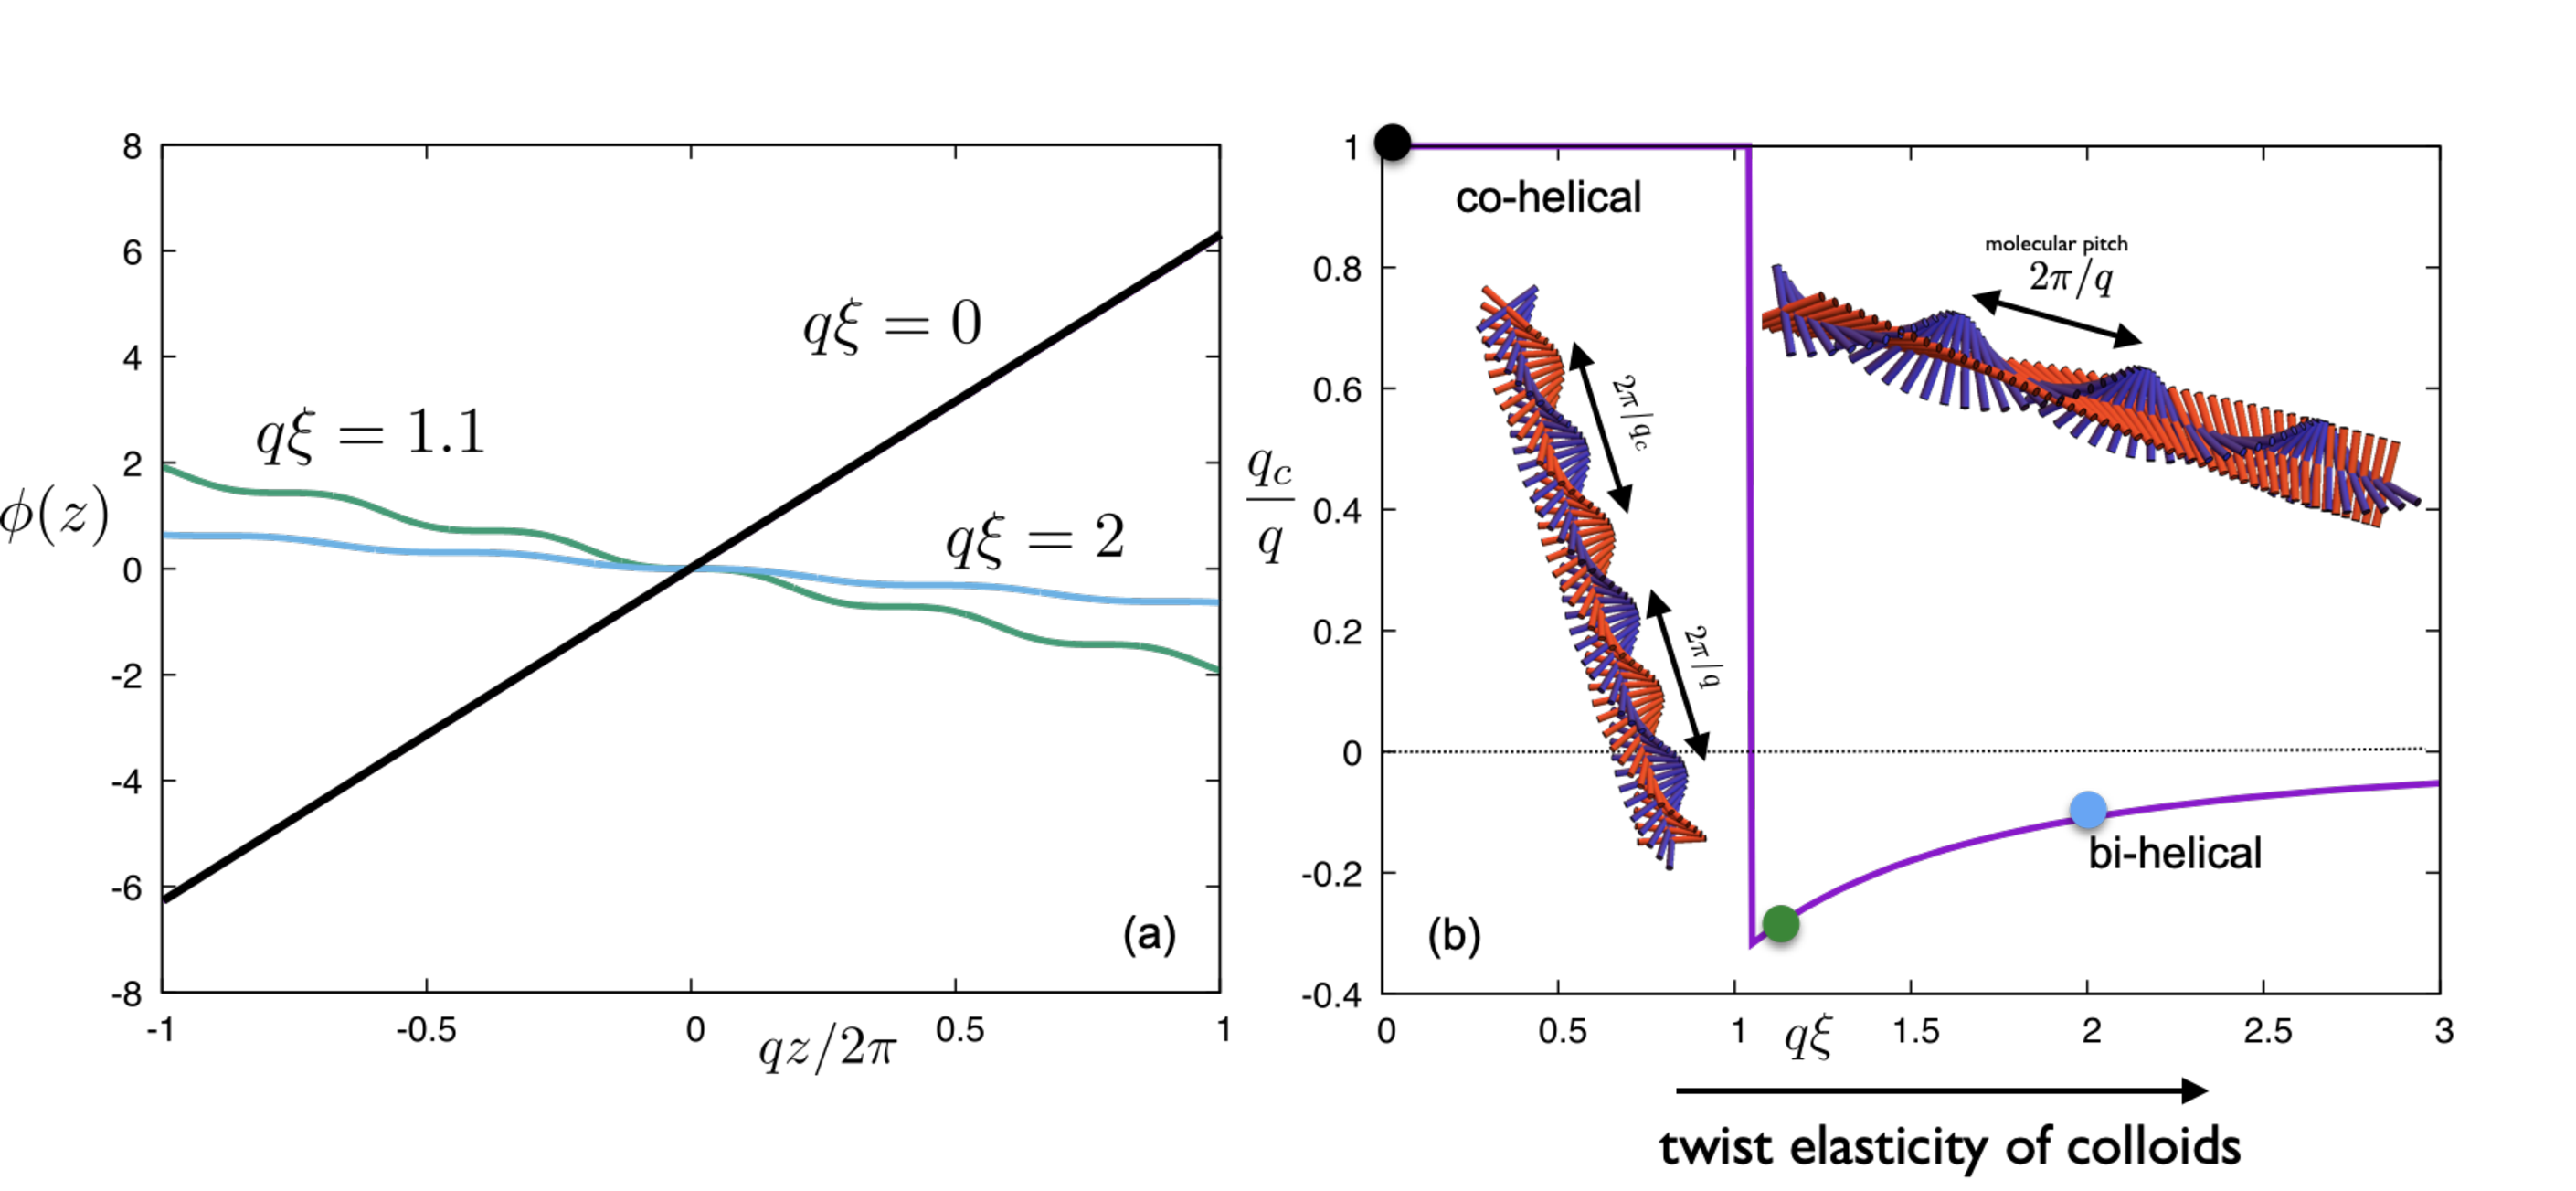
\includegraphics[width =  \columnwidth]{figures/chapter-4/bihelical}
	\caption{ (a) Twist angle $\phi(z)$ of the colloidal director along the helical direction for different strengths of the twist elasticity of the colloids. At weak twist elasticity  ($q \xi <1$) the colloidal director remains co-helical with the cholesteric helix.  At $q \xi >1$ unwinding of the colloidal helix occurs with  ``breathing" instabilities.   (b) Evolution of the pitch $q_{c}$ of the colloidal helix with respect to the cholesteric pitch $q$. Note that in the bi-helical regime the cholesteric and colloidal helices have opposite handedness. The colloidal helix is shown in red, the molecular one in blue.   Colored dots indicate the  state-point corresponding to the breathing profiles in (a). }
	\label{unwind}
\end{figure*}


 \begin{figure}
	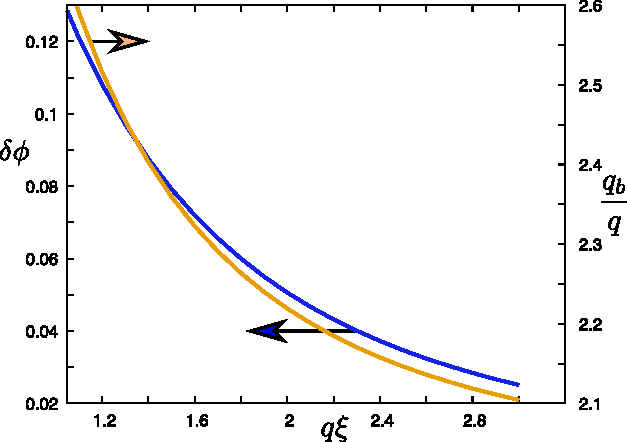
\includegraphics[width = .6\columnwidth]{figures/chapter-4/fluctuations}
	\caption{ Amplitude $\delta \phi$ and periodicity $q_{b}$ of the ``breathing" instabilities encountered in the bi-helical state in \fig{unwind}b as a function of the twist elastic strength $q \xi$. }
	\label{fluc}
\end{figure}

Another common solution that is associated with the sine-Gordon equation is the soliton. Taking the boundary conditions $\varepsilon^{\prime}(\pm \infty) = 0$ and $\varepsilon(\infty) - \varepsilon(-\infty)  = \pi$. The solution for the single soliton can be obtained in analytical form  \cite{kamien2001order}:
\beq
\phi(z) =  qz \pm \frac{\pi}{2} \pm 2 \arctan \left [ \tanh \left ( \frac{z - z_{0}}{R_{s}} \right ) \right ]
\eeq
where $ R_{s} = 2^{1/2} \xi$ defines the soliton width and $z_{0}$ the arbitrary position of its centre along the cholesteric helix. The $-$ solution refers to an anti-soliton. In achiral liquid crystals such as our colloidal subsystem, the (anti-)solitons are unstable with respect to the uniform background (i.e. the co-helical state). The dimensionless free energy difference between the soliton and the co-helical state is  $\tfrac{\Delta Fq}{ A \sigma} = q \xi (2^{3/2} + \pi q\xi)$. However, once they are formed the solitons are metastable and cannot simply relax to the co-helical state without locally destroying nematic order.

From the scaling expression \eq{k2odijk} for the twist elastic constant of rods proposed in the Appendix we find that the soliton width $\sim \xi$ is independent of rod concentration. However, the solitons would be unrealistically small as $\xi $ turns out to be of the same scale as the width of the individual rods, namely  $\xi \sim 70 nm$ for long rods ($L \sim 3 \mu m$ and $D \sim 30 nm$ and $W_{0} = 10^{-5} J/m^{2}$).


\subsection{Effect of rod chirality}

It is well known that conventional (non-hybrid) chiral liquid crystal subject to a uniform electromagnetic field perpendicular to the helical axis may form stable solitons provided that the nematogens are sufficiently chiral \cite{lam2012solitons,ackerman2014two,wu2022hopfions}.  In fact, our rods must have some intrinsic chirality in view of the decoration of helical disclinations imparted by the cholesteric environment, as demonstrated in the previous chapter. The effect of chirality is easily accounted for by an additional free energy \cite{gennes-prost}:
\begin{align}
\frac{F_{\rm chiral}}{A} &= K_{t} \int d z  (\bn(z) \cdot \partial \times \bn(z) )=  K_{t} \int d z (\partial \phi(z) )
\end{align}
with $K_{t}$ denoting the strength of the chiral interactions between the rods. It is customary to identify $K_{t} =q_{r} K_{2}$ where $q_{r}$ would be the pitch of a chiral nematic formed by the rods {\em alone}. In general, $q_{r}$ differs from the pitch $q$ of the cholesteric helix $q$ although a subtle coupling between the two is expected. We stress that $q_{r}$  is a purely hypothetical variable since the rods would not be chiral in the absence of surface anchoring effects imparted by the cholesteric solvent.
Since the chiral contribution is linear in the gradient of $\phi$, the Euler-Lagrange equation \eq{nlde} associated with the total free energy remains unchanged. The boundary conditions now read $\phi(0) = 0$ and $\phi^{\prime}(0) = q_{r}$. If we assume the handedness of the rods to be the same as that of the cholesteric environment, then the main effect of colloid chirality is that the co- to bi-helical transition shifts towards larger $q \xi$. This is a natural consequence of the fact that chirality favors the twisted co-helical state over the (partially) untwisted bi-helical one. Of course, the reverse effect occurs if the rods adopt a handedness that is opposite to that of the cholesteric state ($q_{r} <0$). Then, the transition to the bi-helical state in \fig{unwind}b systematically shifts to smaller $q\xi$ upon increasing the chiral strength $|q_{r}|$.


The free energy between the soliton and the  co-helical state now reads $ \tfrac{\Delta Fq}{ A \sigma} = q \xi [ 2^{3/2}+  \pi q \xi (1-\tfrac{q_{r}}{q})]$. This means that solitons may eventually become stable within the co-helical regime if $\tfrac{q_{r}}{q} > 1 + \tfrac{2^{3/2}}{\pi q \xi}$ which implies that the rods must be very strongly chiral indeed. However, the soliton width is not affected by chirality and remains of the order of the colloid thickness which means that the solitons remain a purely hypothetical scenario, at least within our simple coarse-grained model.

\subsection{Discs}

The case of discs proceeds in an analogous way.  If we assume the same set of basic approximations to hold for the colloidal discs as well, we may start with computing the surface anchoring free energy which takes a simple form  (ignoring irrelevant constants):
\beq
F_{s}[\phi(z)]  =   \begin{cases}
       -\sigma_{\rm \ds H} \cos^{2}[\phi(z) -qz ] &  \textrm{H} \\
        -\sigma_{\rm \ds P} \sin^{2}[ \phi(z) - qz ]  &  \textrm{P}
   \end{cases}
      \label{plahomsdisc}
\eeq
with $\sigma_{\rm \ds H} = \frac{\pi}{4}\rho W_{0}D^{2}\tfrac{J_{1}(qD)}{qD}$ and $\sigma_{\rm \ds P}= \tfrac{1}{2} \sigma_{\rm \ds H}$ describing the two basic anchoring symmetries we consider. Comparing with \fig{fd} we immediately identify the optimal profile $\phi(z) = qz + \phi_{0}$ with $\phi = 0$ (H) and $\phi_{0} = \tfrac{\pi}{2}$ (P) at least for weak to moderate cholesteric pitch $qD < 2$.   Clearly, since the surface anchoring energy has the same basic form  as those previously discussed in \eq{plahoms} for  rods, the director profiles are identical too, provided the  lengthscale $\xi =\sqrt{K_{2}/|\sigma|}$ is taken to be the one appropriate for discs. Using the scaling expression from the Appendix, we find:
\beq
\xi \sim 0.87 c  \sqrt{  \frac{|q|D}{J_{1}(|q|D)}} \sqrt{\frac{k_{B}T}{W_{0}}}
\eeq
which yields about $\xi \approx 80 nm $ for $D = 2 \mu m$ sized discs studied experimentally at a concentration $c = \rho D^{3} =3$, $W_{0} = 10^{-5} J/m^{2}$ and a cholesteric pitch length of $30 \mu m$ corresponding to $qD \approx 0.6$.

For certain values of $qD$ the surface anchoring amplitude $\sigma $may become negative ($\sigma< 0$). In those cases, the phase angles associated with the two anchoring scenarios are simply swapped so that  $\phi = \tfrac{\pi}{2}$ (P) and $\phi_{0} = 0$ (P). By rescaling $\phi(z) \rightarrow \phi(z) - \phi_{0}$ we obtain the  same Euler-Lagrange equation \eq{nlde} with $\sigma \rightarrow | \sigma |$.


\section{Conclusions and outlook}

In this chapter we have theoretically addressed the implications of finite colloid concentration in self-organization of hybrid colloidal-molecular liquid crystals. While at low colloid content the orientation of each colloid is mainly driven my single-particle effect related to surface anchoring and possible surface defects, the phenomenology becomes richer and exciting when colloid-colloid interactions are taken into account. We argue that steric combined with weakly aligning surface anchioring forces may drive liquid-liquid phase separation between two orthorhombic fluid, each with a different colloid concentration and orientational order parameters. In the strong coupling regime, when surface-anchoring-mediated  particle realignement is strong, the colloids impart non-negligible twist elasticity that may stabilize a variety of different bi-helical hybrid LCs in which both molecular and colloidal self-organize along distinctly different helical mesostructures. We also predict the typical colloidal concentration needed to stabilize these structures in experiment. 

At elevated colloid concentration additional interactions could becomes more prominent, for instance those imparted by surface defects and long-range electrostatic forces owing to surface charges residing on the colloids, which will have an impact on the elastic properties generated by the colloids. In fact, one could naively argue  that these could give rise to a significant stiffening of the elastic moduli of the colloidal subcomponent which could lead to a stabilization of bi-helical structures at much lower colloid concentrations than anticipated here.   Clearly, any further quantitative prediction requires a considerable refinement of our analysis beyond the simple steric model considered here.  






%A general solution of \eq{nldereno} under the boundary condition $\varepsilon(0)=0$ can be expressed in terms of the Jacobi amplitude (am) function:
%\beq
%\varepsilon(z) = \textrm{am} \left (qz c_{1}, \frac{2}{- c_{1}^{2} (q\xi)^{2}} \right )
%\eeq
%with $c_{1} > 0$ some unknown constant that needs to be determined from the second boundary condition.







%yields the basic solution $\varepsilon(z) = \varepsilon_{-} \exp(-2^{1/2} z/\xi)+ \varepsilon_{+} \exp(2^{1/2} z/\xi)$. Imposing the boundary condition  $\varepsilon(0) =0$ we find:
%\beq
%\varepsilon(z) = 2\varepsilon_{0} \sinh ( 2^{1/2} z/\xi )
%\eeq
%Since the hyperbolic sine diverges for large $|z|$ the only way to render the solution consistent with $|| \varepsilon ||$ is by setting $\varepsilon_{0} =0$ which means there are no solutions up to linear order in $\varepsilon$.

%Reduction of order leads to
%\beq
%( \varepsilon^{\prime} (z) )^{2} + (q\xi)^{-2} \cos [2 \varepsilon(z)] = C_{1}
%\eeq

\begin{subappendices}
\section{Twist elastic resistance of thin hard needles and discs}

For   hard rods  a tractable analytical expression for the $z-$resolved excluded area is available in the needle limit $L/D \rightarrow \infty$ \cite{poniewierski1988nematic,shundyak2001isotropic}:
\begin{align}
 & {\mathcal A}(|  \Delta z | , \bhu, \bhu^{\prime} ) = -\int d  \Delta \bfr_{\perp} \Phi(|\Delta \bfr |, \bhu, \bhu^{\prime} ) \nonumber \\
 & = 2 L^{2} D |\sin \gamma | \begin{cases}
 0 & |\Delta z| > A+ B \\
 \frac{A + B - |\Delta  z |)}{4 AB } & A - B \leq |\Delta z| \leq A+ B  \\
 \frac{1}{2A} & |\Delta z| < A - B
 \end{cases}
 \label{aexcl}
\end{align}
with $A= \frac{L}{2} | \text{max} ( u_z , u^{\prime}_{z}  ) |$ and $B= \frac{L}{2} | \text{min} (u_{z} , u^{\prime}_{z} ) |$.  We can make headway by realizing that  a rotation of the reference director  only affects the azimuthal angle $\varphi$. More specifically we  have
 ${\mathcal R}(q \Delta z) | \sin \gamma | = \sqrt{1 - (\cos \theta \cos \theta^{\prime}  - \sin \theta \sin \theta^{\prime} \cos (\Delta \varphi - q\Delta z) )^{2}} $
with $\Delta \varphi = \varphi - \varphi^{\prime}$.  Performing the integration over $\Delta z$ we can cast the kernel as a Taylor series in terms of even powers of the colloidal pitch $qL$:
\beq
{\mathcal K}_{q} (\bhu, \bhu^{\prime}) = 2 L^{2} D \sum_{n=0}^{\infty} \frac{(qL)^{2n}}{2n!} a_{2n} (\bhu, \bhu^{\prime})
\eeq
 Note that odd powers in $q$ must vanish since the rods are considered to be achiral. We note that  the immersed rods induce weak distortions of the solvent director which are known to adopt a helical signature that could render the rod-rod interaction chiral.  The angle-dependent factor reads in explicit form:
\begin{align}
a_{2n} (\bhu, \bhu^{\prime}) &=  \frac{(\frac{1}{2}u_{z}+\frac{1}{2}u^{\prime}_{z})^{2n +2} - ( \frac{1}{2}u_{z} - \frac{1}{2}u_{z}^{\prime})^{2n+2}}{ u_{z} u_{z}^{\prime} (2n+1)(n+1)} \nonumber \\
& \times \frac{\partial ^{(2n)} | \sin \gamma |_{q=0}}{\partial \Delta \varphi ^{(2n)}}
\end{align}
and it is easily verified that $a_{0} = | \sin \gamma |$ as required. It is insightful to express the  excess free energy per unit volume in the following way:
\beq
\frac{F_{ex}}{V} = k_{B}T \frac{\rho^{2}}{2} \langle \langle {\mathcal K}_{0}(\bhua, \bhub) \rangle \rangle_{f_{q}} +  \sum_{n=1}^{\infty} \frac{q^{2n}}{2n!} K_{2}^{(2n)}
\label{felast}
\eeq
 The quantities $K_{2}^{(2n)}$ could be interpreted as {\em generalized} twist elastic constants defined as:
\beq
K_{2}^{(2n)} = k_{B}T \rho^{2} L^{2n+2}D \langle \langle a_{2n}(\bhua, \bhub) \rangle \rangle_{f_{q}}
\eeq
for most conventional cholesteric phases the director twist is weak on the scale of the rod ($qL <1$) and the expansion may be truncated after the second term. Furthermore, the  orientation distribution is   unaffected by any director twist so that $f_{q}$ can be approximated by the orientation distribution $f_{0}$ of a non-chiral uniaxial nematic phase. The  quantity $K_{2}^{(2)}$ is then identified as the conventional twist elastic constant for which the microscopic definition reads:
\beq
K_{2}  =K_{2}^{(2)}=  k_{B}T \rho^{2} L^{4}D \langle \langle a_{2}(\bhu, \bhu^{\prime}) \rangle \rangle_{f_{0}}
\eeq
For conventional uniaxial nematic order scaling results exist that relate  $K_{2}$ to the total  rod concentration. Using Gaussian theory Odijk \cite{odijkelastic} found that for asymptotically strong nematic alignment:
\begin{align}
\beta K_{2}D \sim \frac{7}{96} c
\label{k2odijk}
\end{align}
For infinitely thin hard discs a much steeper increase with colloid concentration was found \cite{wensink2018}:
\beq
\beta K_{2}D  \sim 0.606 c^{3}
\eeq
which suggests that lyotropic discotic nematic phases are far more difficult to twist than their rod-based counterparts at equivalent particle concentration (note that $c \gg1$ for most stable nematics).

\end{subappendices}


\clearpage